% -----------------------------------------------
% Vlastní text práce (kapitoly práce)
% -----------------------------------------------

% -----------------------------------------------
\chapter{Mössbauer effect and spectroscopy}
% -----------------------------------------------
Mössbauer effect is a physical effect, which can under certain circumstances occur on atomic nuclei. It consists of recoilless resonance emission/absorption of gamma photons by nuclei of source/absorber with discrete nuclear energy levels. This effect has a special application on the field of material research - the Mössbauer spectroscopy (MS), which is a nuclear experimental technique and a special type of gamma spectroscopy, which uses the appropriate nuclei in studied sample as sonds of local electric and magnetic fields. 

\par
This technique is capable of providing many unique information in material research, geology, chemistry and biology - study of phase and chemical composition of solid materials such as steel, study of local magnetic fields and spin states, in-situ measurements of phase transitions. The main disadvantage of this technique is the fact that there is not an appropriate radiation source for many isotopes. The mayor significance has iron and its isotope $^{57}$Fe with possible radiation source $^{57}$Co (which decays into an excited state of $^{57}$Fe with half-life 271.81 days \cite{co57}), which allows the Mössbauer spectroscopy to be employed on many fields, including the steel industry.

% -----------------------------------------------
\section{Physical concept}

\subsection{Resonace emission and absorption}
In previous chapters was mentioned, that the atomic nuclei are quantum systems with discrete energy levels (analogous to the energy levels of electron shell), thus upon deexcitation or excitation they emit/absorb gamma photon with energy $E_0$ equal to the difference between the levels. For the free, stationary nucleus, the emitted/absorbed energy spectra follow the shape of Lorentzian curve. 

\par
However, these emitted/absorbed energy spectra may be altered - due to the  momentum conservation law, some part of the gamma photon energy is transferred to the  kinetic energy of nucleus, crystal as whole body or is transformed into lattice vibrations (phonons). 
%Due to this fact, the emission and absorption energy spectra may be different and without any overlaps, which prevents the resonance effects from happening.
In the case of free, stationary nuclei, momentum and energy transfers are so high, that the emission and absorption spectra are shifted to different directions by large energetic values, which makes the resonance absorption impossible to observe. However, the nucleus bounded into the crystal lattice is a different case - the crystal as whole body will absorb the momentum. If we consider, that the entire crystal has much larger mass than the nucleus, the energy transfer into crystal's kinetic energy will be very small - the gamma photon energy remains nearly unaltered. Thus this can be considered as recoilless emission/absorption and the energy spectra have overlap, which makes the resonance absorption (Mössbauer effect) observable \cite{moss}.
\par
It also worth mentioning, that there is also a third case - the free nuclei in thermal motion. The velocity of nuclei is guided by Maxwell's statistics and the spectra become widened by Gaussian shape. At higher temperatures, this effect may result into spectra overlap and makes the resonance absorption observable. However, this technique is not much developed yet and has only a small field of application.

\subsection{Interaction of nuclei with local fields}

The nucleus bound inside the lattice surrounded by electrons arranged according to the chemical bonds has perturbed energy levels, which is due to the interaction of nucleus with local electric and magnetic fields -  what results into the fact, that every phase or chemical constitution has its own nuclear emission/absorption spectrum - Mössbauer spectrum. The quantum physics has very-well known computation techniques to describe these variations in energy spectra - the perturbation theory,

\par
The main properties of nucleus which induces the interactions with local electric and magnetic fields are: atomic number $Z$, quadrupole momentum $Q$ and its spin $I$ along with its projections. For spectroscopy there are three main interaction:

\begin{itemize}
\item Electric monopole interaction - the interaction between the protons of nucleus and the s-electrons (which have non-zero probability of being found inside nucleus). It results into isomer shift of energy levels $\delta = E_M - E_0$. The $\delta$ has to be defined with respect to some fixed energy level, for example to the level of the used source. This type of MS spectra is usually referred as a singlet. 
\item Electric quadrupole interaction - the inhomogeneous electric field inside nucleus interacts the quadrupole momentum $Q$ of the nuclei. It results into energy variations with respect to the square of magnetic quantum number $E_Q \sim m^{2}$- the states which allows different values of $|m|$ are splitted into sub-states.

\item Magnetic dipole interaction - the spin $I$ is tied up with magnetic momentum via relation $\mu = \gamma I$, where $\gamma$ is a gyromagnetic ratio. This magnetic momentum interacts with magnetic fields inside nucleus and results into nuclear Zeeman effects - the splitting of the states with respect to possible values of magnetic quantum number $m$. The main difference from the quadrupole interaction is that the spin orientation also matters. The magnetic dipole interaction has a significant role when it comes to study the magnetic properties of materials.
\end{itemize}

Each of these effects can occur separately or simultaneously with the others.


% -----------------------------------------------



\section{Mössbauer spectroscopy}
There are several techniques how to obtain the spectra. In laboratories there are dominant the setups employing transmission or backscattering geometry with sample as an absorber and with the doppler modulation of the gamma photons energy. The transmitted photons or other products developed upon deexcitation are detected by appropriate detector with electronics to accumulate the energy spectra. The energy of gamma photons is varied by the doppler effect - the source is attached to the doppler modulator (transducer), and by the relative velocity of source and absorber the energy of gamma photons is slightly changed.
\par
For transmission geometry the key concept of measurement is that if we irradiate the sample as an absorber gradually by continuous spectrum of gamma rays with energy around the resonance energy $E_0$ ("energy scanning" by the doppler modulator), the gamma photons with energy equal to one of the possible transitions (resonant energies) are absorbed with certain probability. 
%Gamma photons with different energies are due to the low cross section of previously discussed matter interactions mostly transmitted.
The detector is situated behind the absorber and simultaneously measures the number of gamma counts at defined energy step. The minimal counts are measured around the resonant energy. The transmission geometry Mössbauer spectra can be seen on picture \ref{transspec}.

\par
The concept of backscattering geometry is similar in many ways, but the main difference is the detection of the deexcitation products. The sample's nuclei are excited by appropriate gamma photons and in short time, they decay back into the original state with some effects following - reemission of the "original" gamma photons in random direction, emission of electrons from the shell (ejected by deexcitation energy quanta, also called conversion electrons) followed by characteristic RTG or possibly by auger electrons. The detection of electrons and RTG instead of gamma photons have many advantages and disadvantages and for certain application, the usage of backscattering geometry could be more appropriate. For example, the detection of conversion electrons could handle the surface characterization of the sample due to the lesser transmittance of electrons when comparing to gamma photons.


\par
There are also different setups - irradiation by synchrotron radiation (which can produce continuous gamma spectra with high iluminance), using the sample as an source etc.



\section{$^{57}$Fe spectroscopy}

One of the isotopes, on which we are capable to observe a Mössbauer effect is $^{57}$Fe. As a source is used $^{57}$Co, which decays into second excited state of $^{57}$Fe by electron capture. The new $^{57}$Fe nuclei can deexcite itself by two ways (see fig. \ref{Fe57scheme}) - by direct deexcitation onto ground state by emitting 136.5 keV photon or by deexcitation onto the first excited state by emitting 122.1 keV photon and after short lifetime emits 14.4 keV photons (or other possible conversion products) when falling into ground state. The $^{57}$Fe spectroscopy in transmission geometry is based on detection of the 14.4 keV gamma photons. This thesis is mainly devoted to the application of semiconductor detectors for the detection of these 14.4 keV gamma photons. The $^{57}$Fe spectroscopy can also be performed in backscattering geometry by the detection of the conversion electrons or RTG photons with energies around 6.4 keV.

\begin{figure}[H]
 \centering
 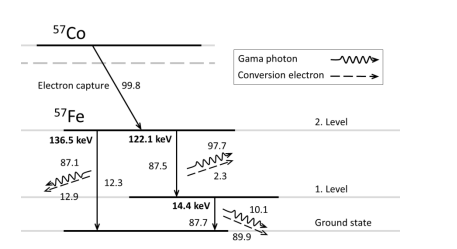
\includegraphics[scale=0.75, angle = 0]{./pictures/Fe57}
 \caption{Decay scheme of $^{57}$Co, taken from \cite{NOVAK2016thesis}.}
 \label{Fe57scheme}
 
\end{figure}


The entire spectrometric setup consist of several parts:
\begin{itemize}

\item Source of 14.4 keV gamma - $^{57}$Co radioctive nuclei built-in crystal lattice (mostly in a rhodium matrice). The source is attached to the transducer.
\item Transducer for doppler modulation. It mostly consists of two coils surrounded by permanent magnets - one for setting the velocity of the source and second for the velocity measurement. The system is driven by PID or MPC controller for precise velocity and energy control. The velocity can be either constant or with constant/varying acceleration.

\begin{figure}[H]
 \centering
 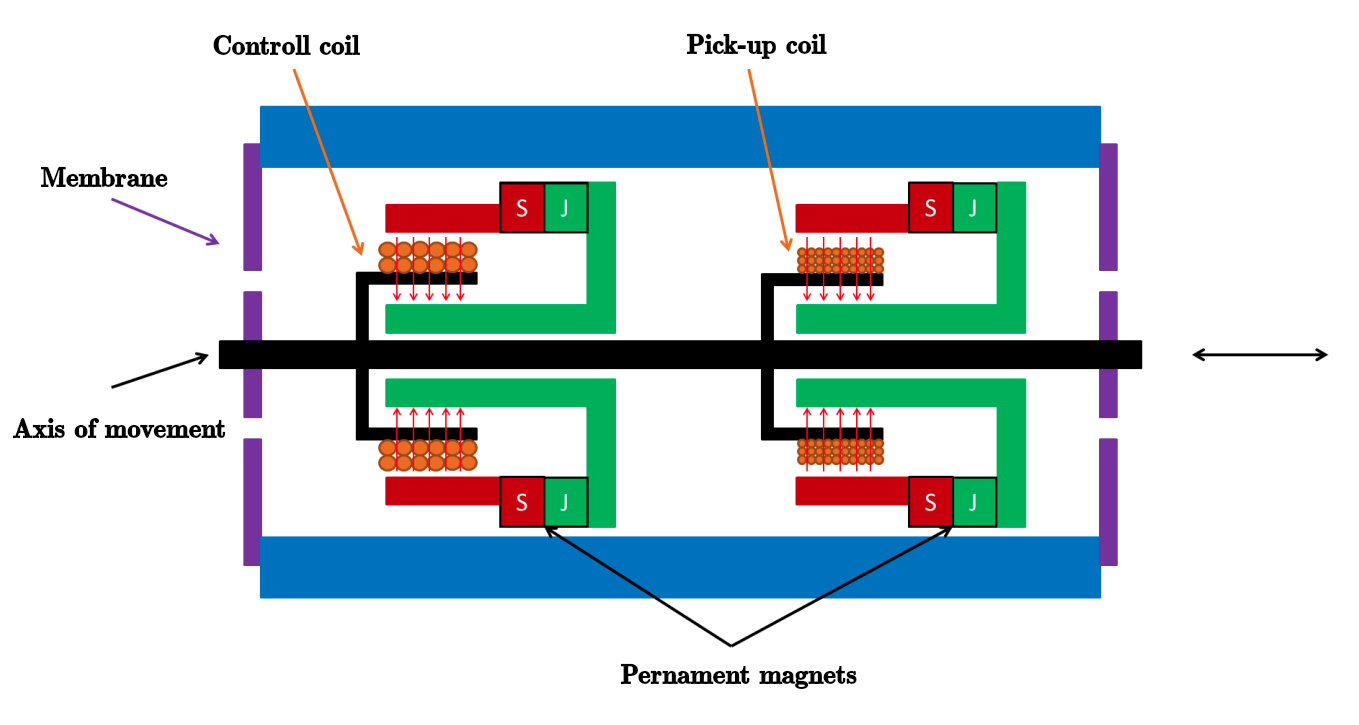
\includegraphics[scale=0.4, angle = 0]{./pictures/transducer}
 \caption{Transducer, taken from \cite{STEJSKAL2019thesis}.}
 \label{transducer}
 
\end{figure}

\item detector of transmitted/backscattered gamma radiation, conversion electrons or RTG along with readout and evaluation electronics including amplifiers, SCA's, MCA's etc. It is also necessary to consider, that the already mentioned conventional detectors have not sufficient energy resolution to distinguish the energy of perturbed states. Because of that, the count rates are synchronised with the velocity signal (actual modulated energy), which is used to address the channels for spectra accumulation. 
%The other approach is to address the channels by precise timing.

\end{itemize}
The functional diagram can be seen on fig. \ref{spectrometric setup}.

\par
It is also necessary to consider, that the $^{57}$Fe isotope have relative abundance only $2.21 \%$ \cite{compounds}. Although this fact, the spectra are still measured with very respectable precision and efficiency, which makes the Mössbauer spectroscopy very sensitive measurement method.

\section{MS spectra quality parameters}
The MS spectra shape can be modelled by Lorentzian curves. The singlet spectra in transmission geometry can be modelled by a single Lorentzian curve in the following form:

\begin{equation}
\begin{aligned}
L(v) = -I\frac{(\frac{\Gamma}{2})^2}{(v - v_0)^2 + (\frac{\Gamma}{2})^2} + B
\end{aligned}
\label{lor}
\end{equation}

Where $I$ is the amplitude, the $\Gamma$ is the FWHM, and the $B$ is a background level. The Lorentzian in this form has the associated area $A$ equal to:

\begin{equation}
\begin{aligned}
A = \pi I \Gamma
\end{aligned}
\label{area}
\end{equation}

There are two properties of MS spectra which characterize its quality: SNR and the Effect $E_{\textrm{MS}}$. They can be calculated from spectra parameters by following equations:

\begin{equation}
\begin{aligned}
\textrm{SNR} = \frac{I}{\sqrt{B}}
\end{aligned}
\label{SNR}
\end{equation}

\begin{equation}
\begin{aligned}
E_{\textrm{MS}} = \frac{I}{B}
\end{aligned}
\label{effect}
\end{equation}



% %%%%%%%%%%%%%%%%%%%%%%%% End of file %%%%%%%%%%%%%%%%%%%%%%%%
